\documentclass[10pt]{article}
\usepackage[margin=.75in]{geometry}\usepackage{amsmath,amssymb,tikz,hyperref}
\setlength{\parindent}{0pt}\setlength{\parskip}{5pt}
\begin{document}
\textbf{Reduced polynomial validity under normalization}\hfill2026-10-31\\T-1140. Producer proof packet; independent source-fidelity review pending.
\section*{Checked construction}
For a field $K$ and $a\ne0$, set $T_n(p)=a^{-n}p(aX+b)$. Degree and natural degree are preserved. For monic $u$, $T_{\deg u}(u)$ is monic. Together with the preceding congruence result, this proves preservation of
\[u\text{ monic},\quad\operatorname{natDegree}(u)\le2,\quad\deg v<\deg u,\quad u\mid f-v^2.\]
The ordinate bound uses $\deg0=\bot$, so the identity $(1,0)$ is included. No characteristic restriction is added beyond the field and nonzero-scale hypotheses.
\begin{center}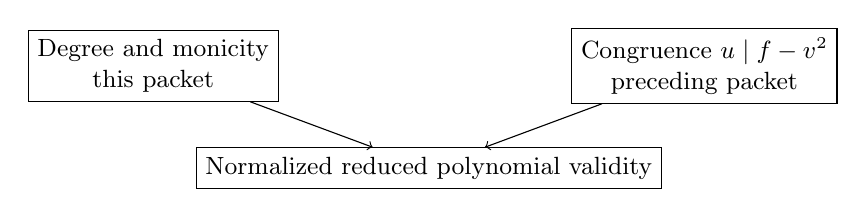
\begin{tikzpicture}[every node/.style={draw,align=center,font=\small}]
\node (a) at (0,0) {Degree and monicity\\this packet};
\node (b) at (7,0) {Congruence $u\mid f-v^2$\\preceding packet};
\node (c) at (3.5,-1.3) {Normalized reduced polynomial validity};
\draw[->](a)--(c);\draw[->](b)--(c);
\end{tikzpicture}\end{center}
\section*{Controls and readback}
Seven main declarations and eleven controls receive separate named axiom readback. With $a=2,b=3$, the exact quadratic control is $T_2((X+1)^2)=(X+2)^2$. Omitting support scaling gives leading coefficient4 and fails monicity. The identity and $(X,1)$ on $f=X^5+1$ satisfy validity and transport correctly. Equal support/ordinate degrees and nonmonic $2X$ are rejected.
\section*{Source correspondence}
\texttt{three\_leads.rs}:945--980 slices support through stored degree$d$ and ordinate strictly below$d$; its validator checks $d\le2$, leading slot1, and empty remainder. \texttt{genus2\_model\_gate.rs}:14--56 retains$d$ and uses scales$a^d,a^3$. This theorem preserves the intended polynomial conditions. Literal vector loops, trim/remainder implementation, machine arithmetic and geometric divisor-class transport remain separate bindings.
\section*{Receipts and scope}
The initial compile failed on missing imports/lemma names. A partial cache overlay then failed module lookup. The third main attempt passed after building a private union from existing cached files. Three added modules and inherited dependencies are hashed; no cache build or download. Two control attempts failed on mapped rational constants/lemma naming; the third passed. Raw failures remain available.

Standardized status, proof sources, full dependency bindings and custody records accompany the packet. Existing compiled Lean dependencies remain in the trust boundary. No independent binary rechecker or semantic review is claimed.

Primary reference: \href{https://leanprover-community.github.io/mathlib4_docs/Mathlib/Algebra/Polynomial/Degree/Lemmas.html}{Mathlib polynomial degree lemmas}, compared with pinned sources. No scientific campaign, enumeration, timing or cost ratio; expired limits unchanged. Diagram shows proof dependencies, not performance.
\end{document}
